% !TEX root = ../thesis.tex
\chapter{基于自适应相似性矩阵的无监督度量学习}
\section{引言}
数据在数据空间中的空间分布学习一直是一个困难的问题。经验上,数据往往分布在高维空间的一个低维流形上,而不是完全随机分布。这导致了不同标签的数据之间可能有较近的欧氏距离。这种分布特性会对基于传统欧氏距离度量的分类或聚类算法的效果产生影响。一个较好的选择是构建一个能够保持数据对之间局部近邻结构的低维映射。

事实证明,度量学习相对于最近邻方法和其他依赖于距离的算法具有巨大优势。在早期的度量学习工作中,文献\parencite{xing2002distance}提出了利用辅助信息的度量学习的框架。这个学习框架的目的在于,通过学习一个距离度量矩阵缩小相似数据之间的距离并同时拉大不相似数据之间的距离。文献\parencite{weinberger2005distance}在支持向量机中将度量学习应用于基于铰链损失的凸优化分类问题。
文献\parencite{davis2007information}提出了基于信息论观点的距离度量学习。他们的工作将度量学习问题表述为在距离函数约束下两个多元高斯分布之间的微分相对熵最小化。后续有大量的扩展度量学习的工作\cite{liu2015low,qian2015fine}以及全面的概述总结文献\cite{yang2006distance,kulis2012metric}被发表。

另一方面,谱聚类方法是一类基于矩阵特征分解的聚类方法,该类方法在很多具有挑战性的真实世界数据集上表现出了非常优异的性能。在最近几十年间,一系列经典的谱聚类方法被提出,例如:多维标度法(Multidimensional Scaling,MDS)\cite{cox2000multidimensional},局部线性嵌入(Local Linear Embedding,LLE)\cite{roweis2000nonlinear},等距特征映射(Isomap)\cite{tenenbaum2000global},拉普拉斯特征映射(Laplacian Eigenmaps)  \cite{belkin2001laplacian}和变种的谱聚类\cite{ng2002spectral}。

上述提到的谱聚类算法有三点不足之处。第一,这些谱聚类算法只提供了训练数据的嵌入映射,对样本外数据(out-of-sample)的计算比较困难。第二,这些算法的复杂度依赖于数据点数量,相对比较耗时,可扩展性不强。第三,谱聚类算法的稳定性高度依赖于相似性图(affinity graph)的鲁棒性。
为缓解上述谱聚类中存在的问题,大量重要的研究进展被提出\cite{bengio2004out,niyogi2004locality,fowlkes2004spectral,yan2009fast,chen2011large,pavan2007dominant,premachandran2013consensus,zhu2014constructing,nie2014clustering}。局部保持投影(Locality Preserving Projections, LPP)\cite{niyogi2004locality}引入了一种由拉普拉斯特征映射得到的线性投影方法。他们的工作提供了一种嵌入映射的线性近似,该线性近似可以减少计算复杂度并可以简单地实现样本外数据的扩展。线性嵌入提供了一种度量学习角度下的谱聚类方法。文献\parencite{nie2014clustering}提出了自适应近邻投影聚类(Projected Clustering with Adaptive Neighbors,PCAN)算法,该算法将点对之间的相似性作为一个额外的待求解变量并且通过对图拉普拉斯(graph Laplacian)矩阵的秩设置惩罚项以限制相似性矩阵的连通区数量。基于这个框架,PCAN算法交替地更新相似性矩阵和投影。经验上,流形嵌入方法的效果依赖于相似性矩阵的鲁棒性。图\ref{fig2:affMat}给出了MNIST数据集\cite{lecun1998gradient}的子集在理想情况下及不同近邻数量下的热力核相似性矩阵。从图中可看出广泛使用的$k$-NN($k$ nearest neighborhood)热力核中存在大量的噪声。虽然一些相似性学习的方法已经被提出,选择合适的相似性矩阵的问题依然有待解决。

\begin{figure}[t]
	\centering
	\bisubcaptionbox{理想的相似性矩阵}%
					{Ideal affinity matrix}
					[0.3\textwidth]{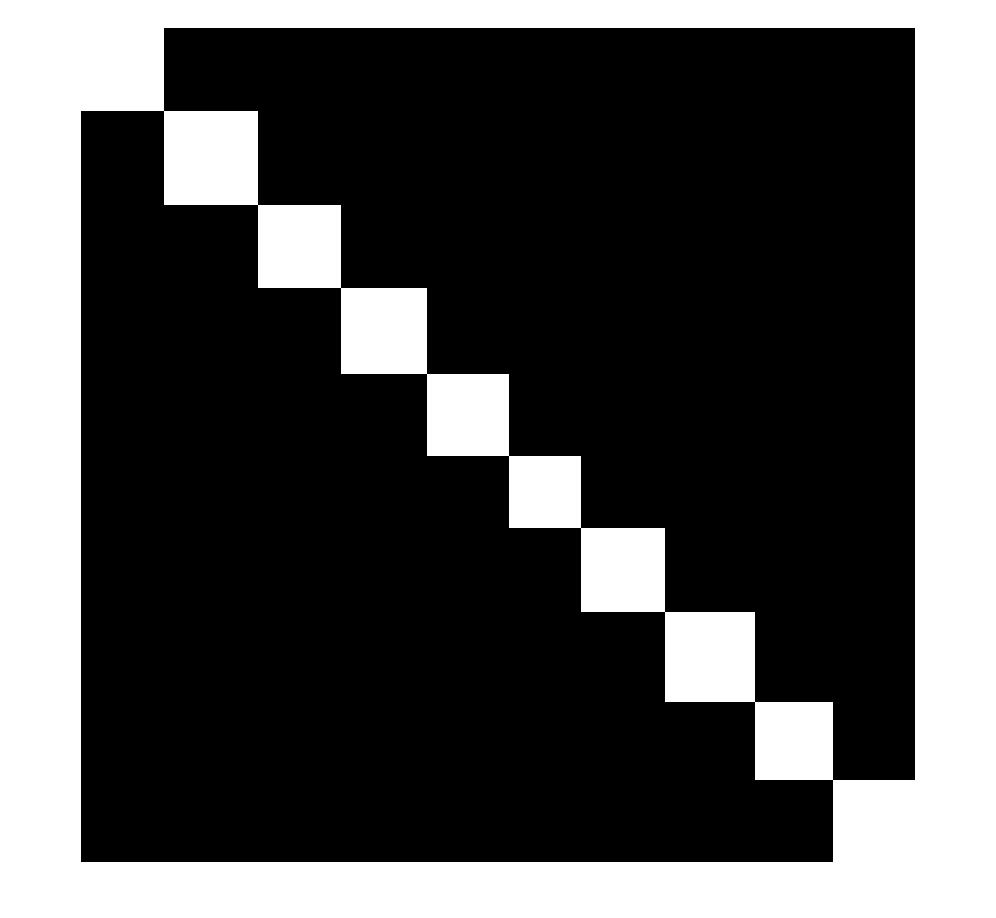
\includegraphics[width=0.3\textwidth]{chap2/k1.jpg}}
	\hspace{1em}
	\bisubcaptionbox{$k=100$下的热力核相似性矩阵}%
					{Affinity matrix of heat kernel with $k=100$}
					[0.3\textwidth]{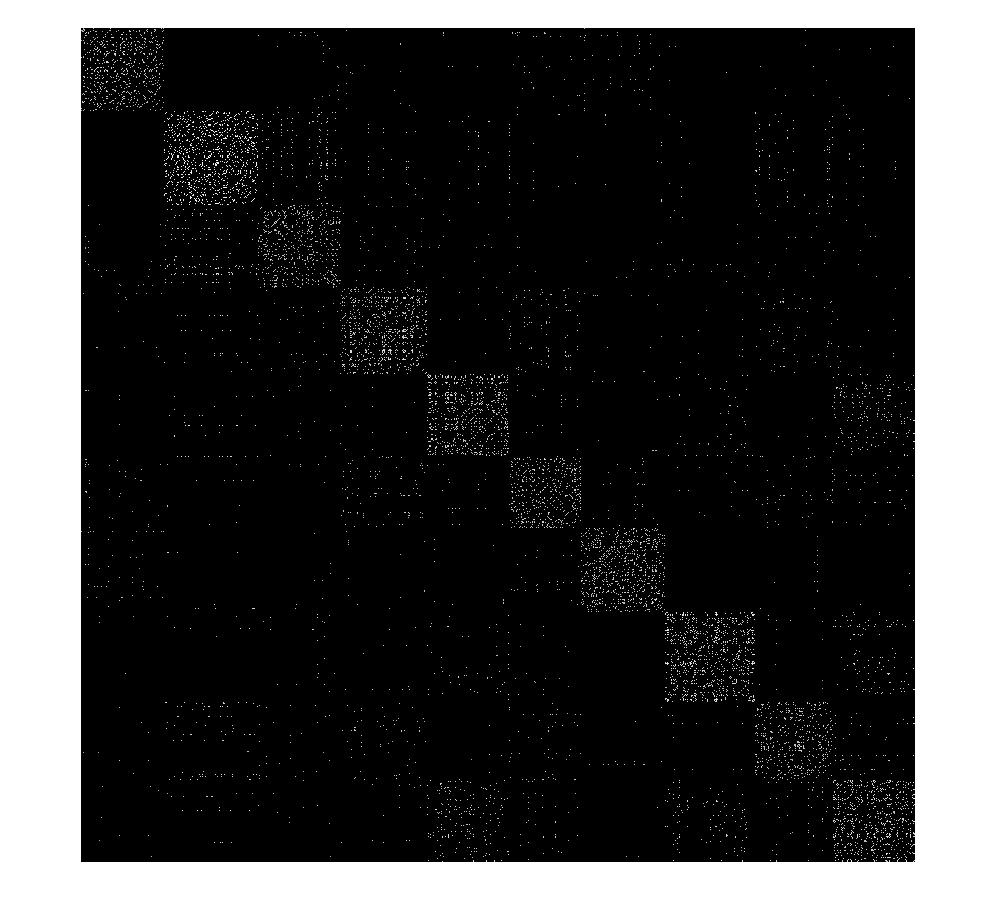
\includegraphics[width=0.3\textwidth]{chap2/k100.jpg}}
	\hspace{1em}
	\bisubcaptionbox{$k=1000$下的热力核相似性矩阵}%
					{Affinity matrix of heat kernel with $k=1000$}%
					[0.3\textwidth]{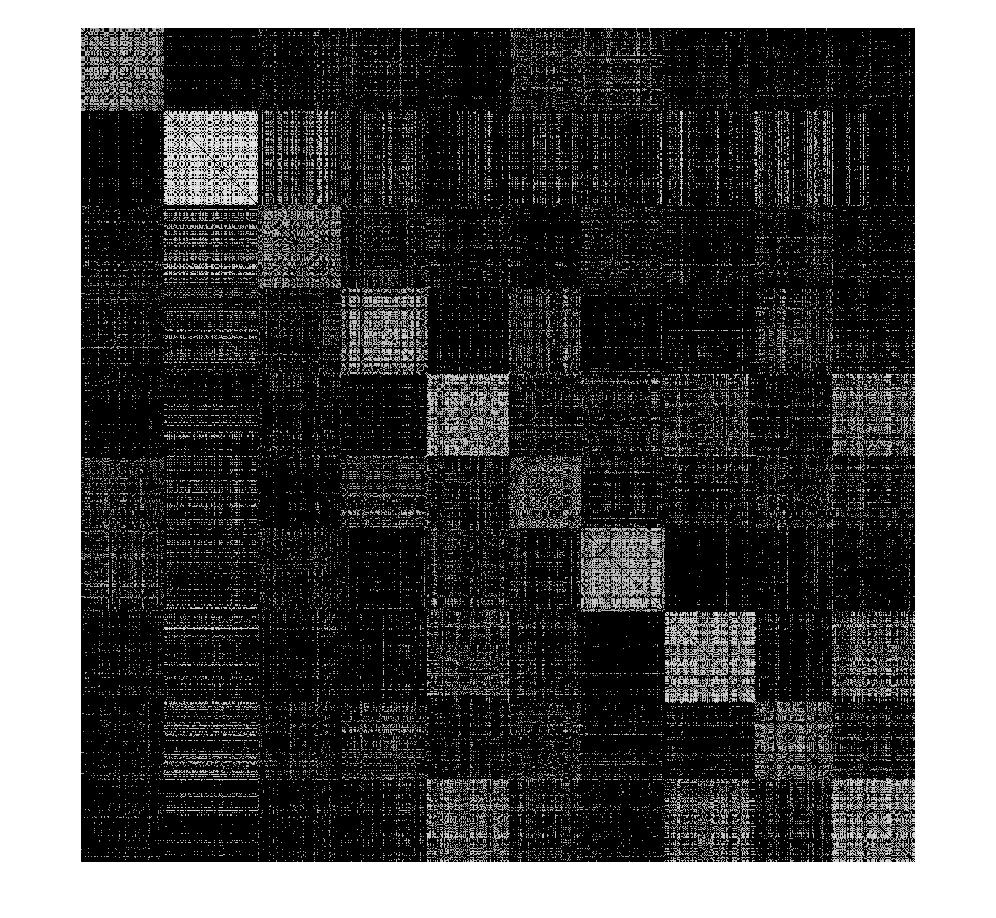
\includegraphics[width=0.3\textwidth]{chap2/k1000.jpg}}
	\bicaption{MNIST子集在理想情况及不同近邻数量$k$下的相似性矩阵}
			  {Ideal affinity matrix and affinity matrices with different neighborhood size $k$ on a subset of MNIST}
  	\label{fig2:affMat}
\end{figure}

本章所提出的方法的目标在于,针对谱聚类的线性近似,在最小的时间消耗下,提取更具有自适应性的相似性信息。这类信息将会更多地考虑局部性保持(locality preserving)这个优化目标,而不仅仅是图像间的距离。受到可扩展谱聚类和数据相似性学习方向上的研究成果\cite{chen2011large,nie2014clustering}的启发,本章提出了一个新颖的自适应相似性矩阵(Adaptive Affinity Matrix,AdaAM)方法。该方法的相似性矩阵相对稠密并可以同时捕捉到全局及局部信息。特别地,AdaAM将相似性矩阵分解成两个相同的低秩矩阵的乘积。作为文献\parencite{ng2002spectral}中描述的理想情况,如果我们假设同一个类内的点对特征极为相似,则相似性矩阵可能会形成一个低秩矩阵。本算法采用与谱聚类方法相似的优化方法对分解后的矩阵进行优化求解。优化得到的相似性图作为最终结果前的中间态相似性矩阵。通过合并基于热力核获得的$k$-NN相似性图和中间态相似性矩阵,AdaAM采用朴素的谱聚类求解方法计算出一个最终的自适应相似性矩阵。我们将LPP方法作用于此特定的相似性矩阵上进行数据投影,以获得一个用于聚类的距离度量。

在本章中,我们将通过在图像数据集上的聚类实验展示所提出方法的有效性和高效性。第 \ref{sec2:Exp}节通过对本章提出的算法和基于$k$-NN的拉普拉斯特征映射\cite{belkin2001laplacian}以及其他最先进方法进行对比展现了AdaAM方法在具有挑战性的数据集上的聚类效果具有明显优势。


\section{自适应相似性矩阵学习}
在本节中,我们首先对本节采用的数学符号进行说明,其次介绍中间态相似性矩阵的计算方法,然后描述最终自适应相似性矩阵的获取方式,最后对算法流程中的稀疏化策略进行介绍。
\subsection{符号说明}
在本章中,我们以大写英文或希腊字母代表矩阵,小写字母代表向量。所有元素全部为$1$的向量用$\bf{1}$表示。$H$表示中心化矩阵(centering matrix),其定义为:$H = I-\frac{1}{n}\bf{1}\bf{1}^T$。原始数据矩阵以$X \in \mathbb{R}^{n\times d}$表示,其中$n$为数据点的数量,$d$为数据维数。本章中将特别地假设数据矩阵$X$为零均值列归一化矩阵,即$X = HX$。符号$x_i$表示数据矩阵$X$中的第$i$个数据点向量。我们用$A$表示线性投影,相应的距离度量矩阵表示为$M = A^TA$。因此,在该度量矩阵下的距离定义为$dis_m(x_i, x_j) = (x_i - x_j)^TM(x_i - x_j)$。我们将$k$-NN热力核矩阵表示为$W \in \mathbb{R}^{n \times n}$:
\begin{equation}
	w_{ij} = \begin{cases} \mathrm{exp}(-\frac{\|x_i-x_j\|_{2}}{t}), \; &x_i\in\mathcal{N}_k(x_j)\;\mathrm{or}\; x_j\in\mathcal{N}_k(x_i);\\
		0, &\mathrm{otherwise.}\end{cases}          
\end{equation}
此处,$\mathcal{N}_k(x)$表示数据点$x$的 $k$ 个最近邻的集合,我们延续了文献\parencite{niyogi2004locality}中对时间参数$t$的设定。相应的拉普拉斯矩阵表示为$L=D-W$,其中$D$为对角权重矩阵:$d_{ii} = \sum_j w_{ij}$。我们对中间态增量矩阵及最终自适应相似性矩阵都采用$\Delta$表示,相应的对角权重矩阵和拉普拉斯矩阵分别表示为$D_\Delta$和$L_\Delta = D_\Delta-\Delta$。

\subsection{中间态相似性矩阵}
我们将提出的AdaAM算法分为两个部分,分别是中间态相似性矩阵和最终自适应相似性矩阵。本节将对其中的中间态相似性矩阵部分的生成进行介绍。对于第$i$个数据点$x_i$,我们使用相似度$\delta_{ij}$对任意的数据点$x_i$和数据点$x_j$进行连接。由于希望任意两个数据点之间较近的欧氏距离能导致较大的数据点相似度,我们的目标为通过选择最优的相似度$\delta_{ij}$在特定合适的约束下最小化下述的目标函数,
\begin{equation}
	\mathop{\mathrm{min}} \sum_{i,j}^{n} \|x_i-x_j\|_2^2\;\delta_{ij},
\end{equation}
在这里,$\delta_{ij}$表示中间态相似性矩阵$\Delta$中第$ij$个元素。

不同于PCAN算法\cite{nie2014clustering}在$\delta_{ij}$上增加稀疏约束后直接进行优化求解,我们首先基于图拉普拉斯矩阵对该目标函数公式进行变形,
\begin{equation}
	\mathop{\mathrm{min}}\; tr(X^TL_\Delta X).
	\label{eq2:Delta}
\end{equation}

由于在通常情况下图拉普拉斯矩阵为半正定矩阵,因此一个直观又看似可行的思路是将拉普拉斯矩阵分解为两个相同矩阵的乘积。在下文中我们将论述该思路并不适用于我们的计算框架。

我们采用$U\in \mathbb{R}^{n\times s}$ 表示一个列正交矩阵,满足$U^TU = I$。我们假设目标矩阵$L_\Delta$可以表示为
\begin{equation}
	L_\Delta = UU^T.
\end{equation}
则在该假设约束下,最终需要求解问题为:
\begin{equation}
	% \begin{split}
		U = \mathop{\mathrm{arg\;min}}_{U^TU=I}\; tr(X^TUU^TX) 
		\Rightarrow U = \mathop{\mathrm{arg\;min}}_{U^TU=I} \;tr(U^TXX^TU).
	% \end{split}
	\label{eq2:simpEigmap}
\end{equation}

如果我们假设矩阵$X$的乘积为矩阵$K$,即$K = XX^T$,则公式(\ref{eq2:simpEigmap})所得为一个简单形式的拉普拉斯特征映射\cite{belkin2001laplacian}。
由此,该优化问题可以通过选择矩阵$K$的多个最小特征值所对应的特征向量形成矩阵进行求解。但是,由于$K$为一个低秩矩阵,一般情况下满足条件$d\ll n$,$K$可以最小化公式(\ref{eq2:simpEigmap})中目标函数的特征向量都存在于数据矩阵$X$的零空间中。
因此,上述问题的最优解不唯一。受LSC(Landmark-based Spectral Clustering)算法\cite{chen2011large}启发,我们将相似性矩阵假设为一个半正定矩阵。不同于对拉普拉斯矩阵进行分解,我们将半正定的相似性矩阵分解为列正交矩阵 $P\in \mathbb{R}^{n\times r}$及其转置矩阵$P^T$的乘积,其中 $r$ 为预期下的矩阵$\Delta$的秩。

由此,我们可以将公式(\ref{eq2:Delta})改写为
\begin{equation}
	% 	\begin{split}
	% 		&\mathop{\mathrm{min}}_{P^TP=I} tr(X^T(D_\Delta-PP^T)X) \\
	% 		&\Rightarrow 
	\mathop{\mathrm{min}}_{P^TP=I} tr(X^TD_\Delta X)+tr(X^T(-PP^T)X),
	% 	\end{split}
	\label{eq2:XLX}
\end{equation}
此处,我们舍弃了连接权重为非负相似度以及图拉普拉斯为半正定矩阵这两个特性。相似性矩阵$\Delta$中的负值连接权重可以用于度量数据点间的不相似度。下面,我们将证明此优化问题的最优解将使$D_\Delta$ 等于 $\bf0$。

\begin{proposition}
	\label{thm2}
	在数据矩阵$X$为列归一化矩阵的条件下,最优化问题(\ref{eq2:XLX})的最优解$P$将使得$D_\Delta=\bf0$成立。
\end{proposition}

\begin{proof}
对于公式(\ref{eq2:XLX})中的第一部分,我们可以将其写为
\begin{equation}
	\begin{split}
		\mathop{\mathrm{min}}\;&\sum_{i=1}^{n} \|x_i\|_2^2\;d_{\Delta ii},\\
		s.t. \;\; &P^TP=I;\\
		&d_{\Delta ii}=(PP^T\textbf{1})_i.
	\end{split}
	\label{eq2:XD}
\end{equation}

令$z=(\|x_1\|_2^2, \|x_2\|_2^2, ... , \|x_n\|_2^2)^T$。此处,取拉格朗日乘子为$\lambda$,公式(\ref{eq2:XD})在一维情况下的优化问题可以表示为
\begin{equation}
	\mathop{\mathrm{min}}\; z^Tpp^T\textbf{1}-\lambda (p^Tp-1)
\end{equation}

最终,最小化优化问题(\ref{eq2:XD})可以被化简为求解问题
\begin{equation}
	\textbf{1}z^Tp=\lambda p
\end{equation}
中最小特征值对应的特征向量。因为矩阵$\textbf{1}z^T$为秩$1$矩阵,所以只存在一个非零特征值$\sum_{i=1}^{n}\|x_i\|_2^2$,同时这也意味着 $\lambda = 0$。由此可知,对于具有任意的小于 $n$的列数且满足优化问题(\ref{eq2:XD})的列正交矩阵$P$,我们可以得出$z^TPP^T\textbf{1}=0$。这个结论等价于
\begin{equation}
	\sum_{i=1}^{n} \|x_i\|_2^2\;d_{\Delta ii} = 0.
\end{equation}

一般性地,对于真实世界数据集中数据点$x_i$,$\|x_i\|_2^2\neq0$恒成立,故能够最小化目标函数(\ref{eq2:XLX})第一部分的最优解$P$ 具有性质$D_\Delta = \textbf{0}$。同时可知,具有性质$D_\Delta = \textbf{0}$的所有$P$的集合构成优化问题(\ref{eq2:XD})的解集。

最小化优化目标函数(\ref{eq2:XLX})的第二部分的矩阵$P$,可以通过求解下述特征问题中最大特征值获得:
\begin{equation}
	\begin{split}
		(XX^T)p = \lambda p
		\Rightarrow {\bf1}^TXX^Tp = \lambda {\bf1}^Tp
	\end{split}
	\label{eq2:Solu}
\end{equation}

由数据矩阵$X$为零均值列归一化矩阵,可以得知$\lambda {\bf1}^Tp = {\bf1}^TXX^Tp = 0$。因而,对于大于$0$的最大特征值,其对应的特征向量$p$总满足${\bf1}^Tp = 0$。将令公式(\ref{eq2:XLX})中第二部分取得最小值的解$P$写为 $P=(p_1,p_2,...,p_t)$,可以得到
\begin{equation}
	%\begin{split}
	{\bf1}^T P = {\bf0} \Rightarrow {\bf1}^T PP^T = {\bf0} \Rightarrow d_{\Delta ii} = 0. %\quad(i=1,...,n)
	%\end{split}
\end{equation}
由此可知,特性$D_\Delta = \textbf{0}$对于公式(\ref{eq2:XLX})第二部分的最优解恒成立,并且该最优解属于公式(\ref{eq2:XD})的解集。所以,公式(\ref{eq2:XLX})第二部分的最优解同时可以使目标函数(\ref{eq2:XD})达到最优。完整的优化问题(\ref{eq2:XLX})的最优解使得
\begin{equation}
	D_\Delta={\bf0}.
\end{equation}
\end{proof}

由命题\ref{thm2}及其证明可知,优化目标函数(\ref{eq2:XLX})可以进一步化简为
\begin{equation}
	P=\mathop{\mathrm{arg\;max}}_{P^TP=I} \;tr(P^TXX^TP).
	\label{eq2:PXXP}
\end{equation}
公式(\ref{eq2:PXXP})的最优解可以通过对数据矩阵 $X$ 的奇异值分解求得,其运算复杂度依赖于数据维度$d$而不是数据量$n$。至此,我们从同时具有相似度和不相似度信息的原始数据分布中获得了中间态相似性矩阵 $\Delta = PP^T$。矩阵$\Delta$所对应的图拉普拉斯矩阵为$L_\Delta = D_\Delta-\Delta =-\Delta $。

为了能够缓解计算中的噪声影响以及矩阵秩减少的问题,我对矩阵$\Delta$进行了稀疏化处理。我们将在第\ref{sec2:sparse}节对稀疏化处理的细节进行进一步讨论。

\subsection{最终自适应相似性矩阵}
在本节中,我们对朴素的线性谱聚类进行公式化,并且给出最终自适应相似性矩阵的求解方法。

在已经求得中间态相似性矩阵$\Delta$的情况下,我们可以通过求解下述问题获得一个线性投影矩阵$A$:
\begin{equation}
	a = \mathop{\mathrm{arg\;min}}_{a^Ta=1}\; tr(a^TX^T(L+L_\Delta)Xa),
	\label{eq2:AXLXA}
\end{equation}
此处,$a$ 为矩阵$A$的一维情况,且$L+L_\Delta$是$k$-NN热力核$W$与中间态相似性矩阵$\Delta$的拉普拉斯矩阵的组合。投影向量$a$可通过求解特征分解问题的最小特征值得到:
\begin{equation}
	X^T(L-\Delta)Xa = \lambda a
\end{equation}

然后,为在给定$A$的情况下求解公式(\ref{eq2:AXLXA})中的$L_\Delta$,我们依照对公式(\ref{eq2:XLX})的变形,将相似性优化问题进行重写并引入线性投影矩阵$A$:
\begin{equation}
	% \begin{split}		
		P = \mathop{\mathrm{arg\;min}}_{P^TP=I}\; \Big( c+tr(A^TX^TD_\Delta XA) 
		+tr(A^TX^T(-PP^T)XA)\Big),
	% \end{split}
	\label{eq2:AXDXA-PXAAXP}
\end{equation}
这里$c=tr(A^TX^TLXA)$,并且我们假设最终自适应相似性矩阵为$\Delta = PP^T$。由于$X$为列零均值的列归一化矩阵,则$XA$同样为列零均值矩阵,特性$D_\Delta = \textbf{0}$依然成立。由此可知,公式(\ref{eq2:AXDXA-PXAAXP})可化简为
\begin{equation}
	P = \mathop{\mathrm{arg\;max}}_{P^TP=I}\; tr(P^TXAA^TX^TP)
	\label{eq2:PXAAXP}
\end{equation}

公式(\ref{eq2:PXAAXP})可以通过对矩阵$A$进行奇异值分解并提取前$r$个最大奇异值对应的左奇异向量(left-singular vectors)进行求解。我们对从公式(\ref{eq2:PXAAXP})求解得到的自适应相似性矩阵$\Delta=PP^T$进行稀疏化处理,由此可以得到稀疏相似性矩阵。

直观来说,我们可以通过对公式(\ref{eq2:AXLXA})和公式(\ref{eq2:PXAAXP})进行交替迭代求解以使目标函数最小化。然而,如图\ref{fig2:itera}所示,在实际计算中,仅在执行一次迭代运算后所得到的自适应相似性矩阵即可取得很好的聚类效果。持续的迭代求解并没有表现出显著的聚类准确率提升。

在一些算法中图节点的权重具有重要作用,同时例如LPP的一类基于归一化割(Normalized Cuts,NCuts)的方法存在依赖于矩阵$D_\Delta$的优化约束条件。然而在我们的算法中有$D_\Delta = \textbf{0}$,因此,我们将由原始$k$-NN热力核计算得到的权重矩阵$D$叠加到求得的自适应相似性矩阵上,以还原损失的权重信息。最后,我们将原LPP算法中的相似性矩阵替换为由AdaAM方法求得的矩阵$\Delta+D$即可求解出线性投影矩阵$A$ 以及距离度量矩阵$M = A^TA$。

\begin{figure}[t]
	\centering
	\begin{subfigure}{0.49\textwidth}
		\centering
		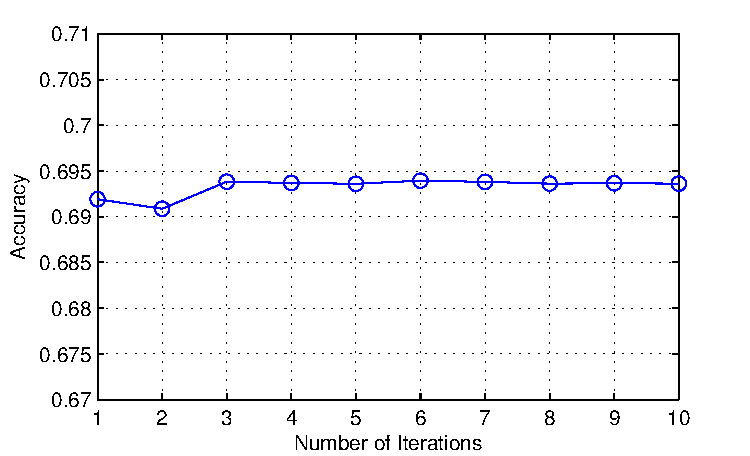
\includegraphics[width=\textwidth]{chap2/itera_data.pdf}
		\caption{}
		\label{fig2:itera}
	\end{subfigure}
	% \hspace{1em}
	\begin{subfigure}{0.49\textwidth}
		\centering
		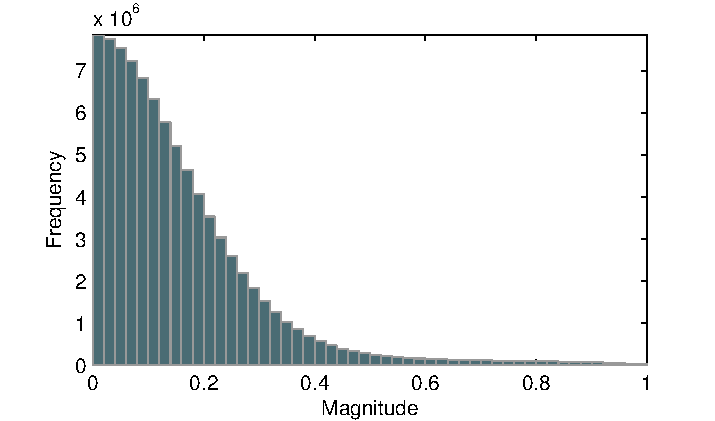
\includegraphics[width=\textwidth]{chap2/delta_hist.pdf}
		\caption{}
		\label{fig2:Hist}
	\end{subfigure}
	\bicaption{a)在数据集USPS上不同的迭代计算次数的聚类效果评价结果。迭代计算所贡献的精度提升小于0.5\%;b)数据集USPS的最终自适应相似性矩阵的元素强度直方图}
			  {a) The evaluation of the clustering performance with different times iterative computation on the data set USPS. The contribution to accuracy made by iteration is less than 0.5\%; b) The histogram of the element magnitude of the final adaptive affinity matrix obtained from data set USPS}
\end{figure}

\subsection{稀疏化策略}
\label{sec2:sparse}

从优化问题(\ref{eq2:PXXP})和(\ref{eq2:PXAAXP})我们可以观察到,矩阵$XX^T$ 和 $XAA^TX^T$都是低秩矩阵。由于上述的优化问题都需要通过矩阵奇异值分解进行求解,所以这个低秩现象将会导致最优解矩阵$P$的列的数量远小于矩阵 $XX^T$ 和 $XAA^TX^T$ 的秩数。这个计算流程将会产生低秩的相似性矩阵,而低秩相似性矩阵会导致我们的算法中的矩阵秩的进一步减小。为避免该矩阵秩持续减小问题的发生,我们在提出的算法中对矩阵实施了稀疏化操作。我们采用的稀疏化策略可以同时缓解数据图中的噪声边问题。

在图\ref{fig2:Hist}中,我们展示了不经过稀疏化处理情况下通过公式(\ref{eq2:PXAAXP})求得的自适应相似性矩阵的元素强度直方图。从图\ref{fig2:Hist}中我们可以观察到,绝大多数的相似性矩阵元素都集中在数值强度较小的范围内,这有效证明了我们对相似性矩阵进行稀疏化处理的合理性。同时,稀疏化处理可以有效的保留住一部分表达能力更强的相似性元素。

受到$k$-NN热力核构造思路的启发,我们对相似性矩阵$\Delta$中的全部元素根据强度大小进行降序排序,只保留其中的前$s$个元素。假设在稀疏化处理后,仅有类内数据点间的相似性被保留下来,不同类间的数据点相似性被删除。在这种情况下,我们考虑到参数$s$的大小应该与聚类的类数成反比,这可以使最终保留下来元素数量近似与图\ref{fig2:affMat}中所示的理想情况下元素数量保持固定比例。参数$s$的计算公式为:
\begin{equation}
	s = \lfloor \frac{n^2}{\alpha c}\rfloor
\end{equation}
此处 $\lfloor \cdot\rfloor$为向下取整函数,$n^2$为矩阵$\Delta$中的元素总数量,$c$为聚类的类数,$\alpha$为一个可调的比例系数。

\begin{algorithm}[t]
	\SetKwInput{KwData}{输入}
	\SetKwInput{KwResult}{输出}
	\caption{自适应相似性矩阵}
	\label{alg2:AdaAM}
	\KwData{数据点 $X \in \mathbb{R}^{n \times d}$;聚类数量 $c$;近邻数量 $k$;降维后维度 $m$。}
	\KwResult{距离度量矩阵 $M$ 和线性投影矩阵$A$。}
	构建$k$-NN热力核矩阵$W$,相应的对角化权重矩阵$D$ 以及拉普拉斯矩阵$L$;\\
	根据公式(\ref{eq2:PXXP}),计算获得列正交矩阵$P$,并求得相应的中间态相似性矩阵$\Delta = PP^T$;\\
	根据公式(\ref{eq2:AXLXA}),求解得到线性投影矩阵$A$;\\
	求解公式(\ref{eq2:PXAAXP}),构造新的$P$矩阵,生成相应的最终自适应相似性矩阵$\Delta = PP^T$;\\
	通过将LPP算法作用于相似性矩阵$\Delta + D$,计算出线性投影矩阵 $A\in\mathbb{R}^{m\times d}$ 及距离度量矩阵 $M=A^TA$。
\end{algorithm}

对于计算中间态相似性矩阵中的第一次稀疏化处理,我们设置$\alpha$为$2.5$,对于计算最终自适应相似性矩阵中的第二次稀疏化,我们将$\alpha$设置为$5$。此处的$\alpha$通过参数搜索确定,并且能够在大多数数据集上给出稳定的表现。

我们在算法\ref{alg2:AdaAM}中对我们所提出的AdaAM算法流程进行了总结。我们在算法实现中将降维后的维度$m$设置为与聚类的类数相同。


\section{实验结果}
\label{sec2:Exp}
在本节中,我们针对所提出算法在图像数据集上的聚类效果、对构建相似性图中的近邻数量敏感性以及算法的运行时间设计了大量的实验,并与其他最先进的算法进行的对比。实验结果验证了所提出的AdaAM算法的有效性、稳定性和高效性。
\subsection{数据集描述}
我们在五个被广泛使用的灰度图像数据集上对所提出的算法及对照算法进行了性能评估:

\begin{figure}[t]
	\centering
	\bisubcaptionbox{UMIST数据集}%
					{UMIST dataset}
					[0.49\textwidth]{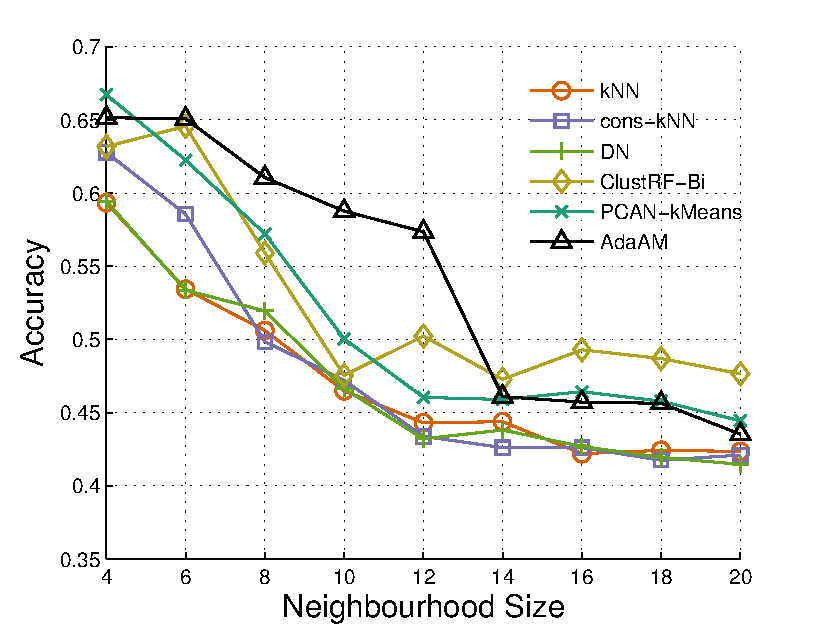
\includegraphics[width=0.49\textwidth]{chap2/sens_UMIST.pdf}}
	\bisubcaptionbox{COIL20数据集}%
					{COIL20 dataset}
					[0.49\textwidth]{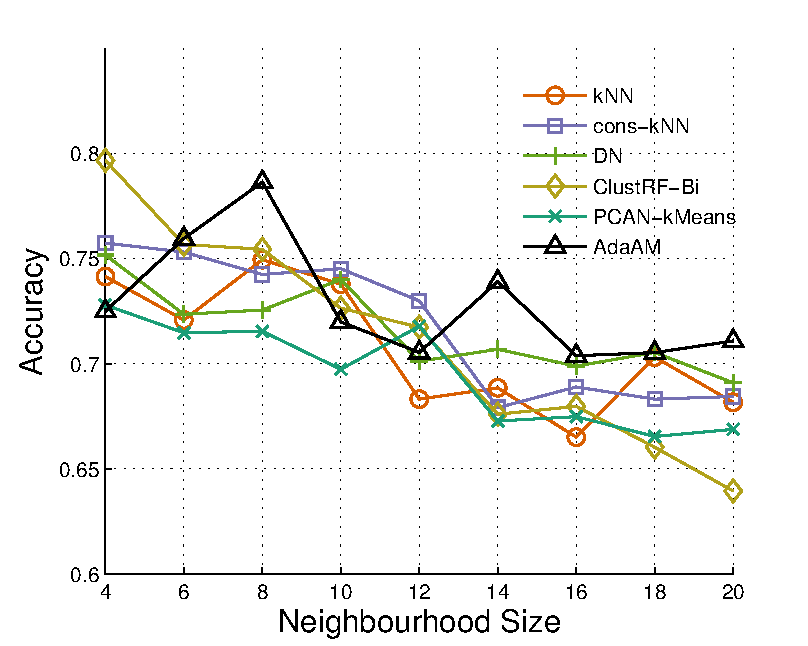
\includegraphics[width=0.49\textwidth]{chap2/sens_COIL20.pdf}}
	\bicaption{在数据集UMIST和COIL20上不同的近邻数量$k$的情况下的算法聚类效果比较}{Clustering results comparison between methods with different neighborhood size $k$ on UMIST and COIL20}
	\label{fig2:Sen}
\end{figure} 

\begin{itemize}
	\item {\textbf{UMIST}}。UMIST人脸数据集 \cite{graham1998characterising}包括20个人的共计575张灰度图片,每张图片尺寸为220$ \times $220像素。在我们的实验中,我们将原图缩小到40$ \times $40像素。
	\item {\textbf{COIL20}}。COIL20数据集\cite{nene1996columbia}包含20个不同物体,共1,440张灰度图片。数据集图片尺寸为32$\times$32像素,图片背景被丢弃仅保留了前景物体。
	\item {\textbf{USPS}}。USPS手写数字数据库\cite{hull1994database}包含了10个数字共计9,298张的灰度图像,图像尺寸为16$\times$16像素。
	\item {\textbf{MNIST}}。MNIST手写数字数据库\cite{lecun1998gradient}训练集包含10类数字共计70,000张灰度图像。图片尺寸为28$\times$28像素。在我们的实验中,我们使用了该数据库训练集中前10,000张图片。
	\item {\textbf{ExYaleB}}。Extended Yale Face Database B(ExYaleB)人脸数据集\cite{KCLee05}由2,414张经过裁剪的人脸图像组成,包含38个个体,每个个体在不同光照下拍摄大约64张图像。在实验中,我们将ExYaleB图像缩小到32$ \times $32像素。
\end{itemize}

在表格\ref{tab2:Data}中,我们总结了五个基准图像数据集的统计量描述。

\begin{table}[t]
	\bicaption{五个基准数据集的统计量描述}{Statistics of five benchmark data sets}
	\label{tab2:Data}
	\centering
		%\begin{sc}
	\begin{tabular}{l c c c}
		\toprule
		数据集 & 实例数目 & 特征维度 & 类别数目\\ 
		\midrule
		UMIST & 575 & 1,600 & 20\\
		COIL20 & 1,440 & 1,024 & 20\\
		USPS & 9,298 & 256 & 10\\
		MNIST & 10,000 & 784 & 10\\
		ExYaleB & 2,414 & 1,024 & 38\\
		\bottomrule
	\end{tabular}
		%\end{sc}
\end{table}

\subsection{对照算法介绍}
我们将所提出的AdaAM方法的聚类效果与本节中介绍的其他相似性学习算法进行了比较。 我们将LPP方法分别应用于通过这些最先进方法生成的相似性矩阵,以获取距离度量矩阵。

\begin{itemize}
	\item \textbf{Con-$k$NN}。Consensus $k$-NNs(Cons-$k$NN)算法\cite{premachandran2013consensus}的目标在于选取更鲁棒的数据点近邻集合。Cons-$k$NN方法通过收集多轮$k$-NN相似性计算中的共识信息,来为数据点近邻集合的选择提供判断标准。
	\item \textbf{DN}。Dominant Neighborhoods(DN)算法\cite{pavan2007dominant}通过在已构建出的相似性图中迭代地选取最大团的方法,实现对相似性矩阵中存在的噪声边的过滤。
	\item \textbf{ClustRF-Bi}。ClustRF-Bi算法\cite{criminisi2012decision,pei2013unsupervised,zhu2014constructing}是ClustRF-Strct\cite{zhu2014constructing}算法的一个计算量较小的特例。由于原始ClustRF-Strct算法在仅有数千个数据实例的情况就需要极大量的计算机内存,我们在本章的实验中采用了这个计算量和内存需求相对可行的特例。ClustRF-Strct提出了一种具有结构感知能力的相似性推断模型,该模型通过利用随机森林进行聚类从而构建数据的相似性图。ClustRF-Bi作为一个特例仅通过随机森林聚类构建二值化的相似性矩阵。
	\item \textbf{PCAN}。文献\parencite{nie2014clustering}提出了Projected Clustering with Adaptive Neighbors(PCAN)方法。由于PCAN是一种可以同时生成线性投影和聚类的算法,所以在结果展示中,我们将PCAN的投影和$k$-means聚类的组合方法表示为PCAN-$k$Means方法,并在表格\ref{tab2:Acc}中显示仅采用PCAN算法生成的聚类结果以供对照参考。
	\item \textbf{$k$-NN}。我们还将所提出的方法与采用$k$-NN热力核相似性矩阵直接进行线性投影的效果进行比较,即采用$k$-NN热力核的LPP算法。我们在后续实验中使用$k$-NN表示这种典型的方法。
\end{itemize}

\begin{figure}[t]
	\centering
	\bisubcaptionbox{USPS数据集}%
					{USPS dataset}
					[0.49\textwidth]{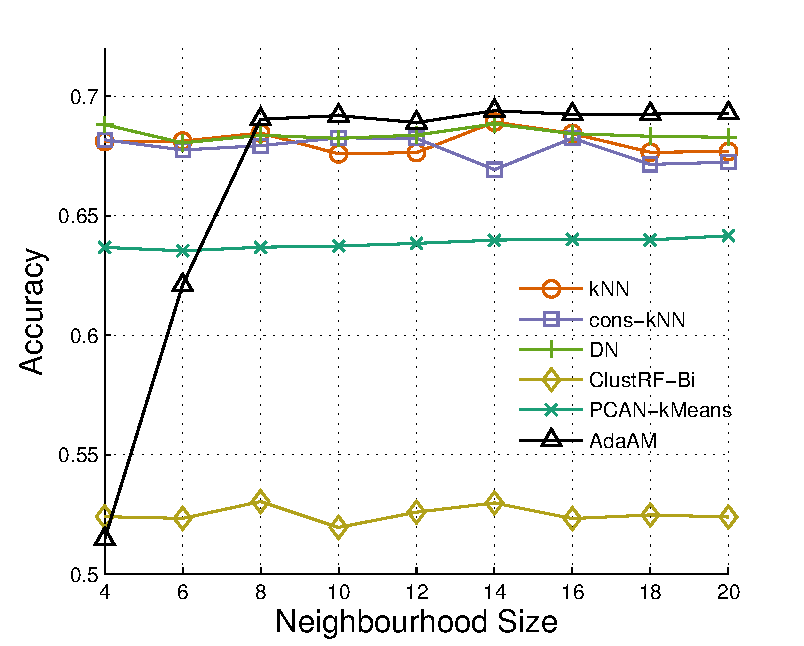
\includegraphics[width=0.49\textwidth]{chap2/sens_USPS.pdf}}
	\bisubcaptionbox{MNIST数据集}%
					{MNIST dataset}
					[0.49\textwidth]{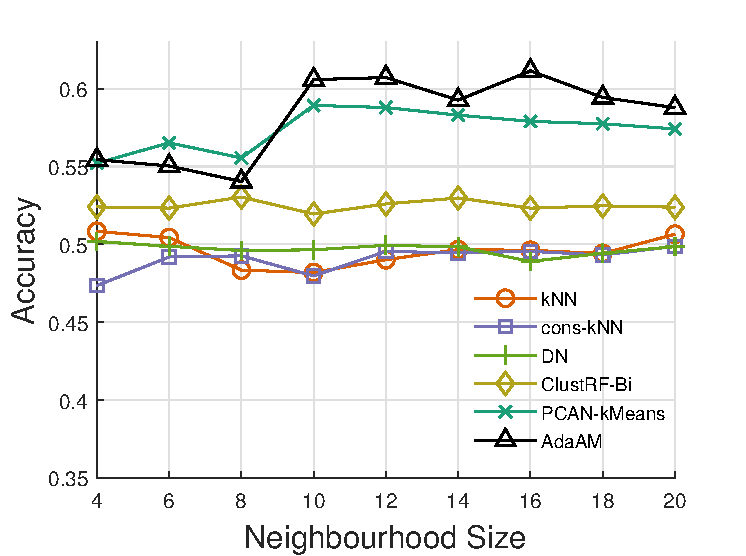
\includegraphics[width=0.49\textwidth]{chap2/sens_MNIST.pdf}}
	\bicaption{在数据集USPS和MNIST上不同的近邻数量$k$的情况下的算法聚类效果比较}{Clustering results comparison between methods with different neighborhood size $k$ on USPS and MNIST}
	\label{fig2:Sen2}
\end{figure} 
% \begin{table}[t]
% 	\bicaption{不同图像数据集上的聚类准确率(\%)}
% 	{Clustering accuracy on different image datasets(\%)}
% 	% \label{tab2:Acc}
% 	\small
% 	\centering
% 	% \begin{small}
% 		%\begin{sc}
% 		\begin{tabular}{llccccccc}
% 			\toprule
% 			& &$k$-NN\cite{niyogi2004locality} &Cons-$k$NN\cite{premachandran2013consensus} &DN\cite{pavan2007dominant} &ClustRF-Bi\cite{zhu2014constructing} &PCAN-$k$Means\cite{nie2014clustering} &PCAN\cite{nie2014clustering}& AdaAM
% 			\\
% 			\midrule
% 			\multirow{2}{*}{UMIST} 
% 			& Avg & 58.16& 60.27& 59.15& 64.63& 53.79& \multirow{2}{*}{55.30}   & \textbf{66.06}\\
% 			& Max& 65.39& 69.22& 66.96& 74.44& 56.52&& \textbf{75.65}\\
% 			\midrule
% 			\multirow{2}{*}{COIL20} 
% 			& Avg & 71.89& 75.53& 71.95& \textbf{76.50}& 72.28& \multirow{2}{*}{81.74}& 74.72\\
% 			& Max& 81.18& 84.31& 82.01& 85.07& 83.75&& \textbf{87.29}\\
% 			\midrule
% 			\multirow{2}{*}{USPS}  
% 			& Avg & 68.25& 68.21& 68.08& 58.74& 64.04& \multirow{2}{*}{64.20}  & \textbf{69.36}\\
% 			& Max& 68.35& 68.34& 68.31& 65.90& 67.95&& \textbf{69.61}\\
% 			\midrule
% 			\multirow{2}{*}{MNIST} 
% 			& Avg & 48.13& 47.88& 49.72& 51.93& 58.93& \multirow{2}{*}{59.83}  & \textbf{60.84}\\
% 			& Max& 48.27& 48.00& 49.76& 52.03& 58.98&& \textbf{61.34}\\
% 			\midrule
% 			\multirow{2}{*}{ExYaleB} 
% 			& Avg& 24.17& 25.63& 24.21& 23.10& 25.74& \multirow{2}{*}{25.89} & \textbf{54.36}\\
% 			& Max& 26.76& 28.75& 27.42& 26.43& 27.63&& \textbf{57.87}\\
% 			\bottomrule
% 		\end{tabular}
% 		%\end{sc}
% 	% \end{small}
% \end{table}
\begin{table}[t]
	\setlength{\tabcolsep}{8pt}
	\bicaption{不同图像数据集上的聚类准确率(\%)}
	{Clustering accuracy on different image datasets (\%)}
	\label{tab2:Acc}
	\centering
	% \begin{small}
		%\begin{sc}
		\begin{tabular}{lcccccc}
			\toprule
			& &UMIST&COIL20&USPS &MNIST& ExYaleB
			\\
			\midrule
			\multirow{2}{*}{$k$-NN\cite{niyogi2004locality}} 
			& Avg & 58.16& 71.89& 68.25& 48.13& 24.17\\
			& Max& 65.39 & 81.18 & 68.35 & 48.27 & 26.76 \\
			\midrule
			\multirow{2}{*}{Cons-$k$NN\cite{premachandran2013consensus} } 
			& Avg & 60.27 & 75.53 & 68.21 & 47.88 & 25.63 \\
			& Max& 69.22 & 84.31 & 68.34 & 48.00 & 28.75 \\
			\midrule
			\multirow{2}{*}{DN\cite{pavan2007dominant}}  
			& Avg & 59.15 & 71.95 & 68.08 & 49.72 & 24.21 \\
			& Max& 66.96 & 82.01 & 68.31 & 49.76 &  27.42\\
			\midrule
			\multirow{2}{*}{ClustRF-Bi\cite{zhu2014constructing} } 
			& Avg & 64.63 & \textbf{76.50} & 58.74 & 51.93 & 23.10 \\
			& Max& 74.44 & 85.07 & 65.90 & 52.03 & 26.43 \\
			\midrule
			\multirow{2}{*}{PCAN-$k$Means\cite{nie2014clustering}} 
			& Avg& 53.79 & 72.28 & 64.04 & 58.93 & 25.74 \\
			& Max& 56.52 & 83.75 & 67.95 & 58.98 & 27.63 \\
			\midrule
			PCAN\cite{nie2014clustering} 
			& - & 55.30 & 81.74 & 64.20 & 59.83 & 25.89 \\
			\midrule
			\multirow{2}{*}{AdaAM} 
			& Avg& \textbf{66.06} & 74.72 & \textbf{69.36} & \textbf{60.84} & \textbf{54.36} \\
			& Max& \textbf{75.65} & \textbf{87.29} & \textbf{69.61} & \textbf{61.34} & \textbf{57.87} \\
			\bottomrule
		\end{tabular}
		%\end{sc}
	% \end{small}
\end{table}

\subsection{参数选择与实验设置}
由于在无监督学习任务中不存在验证数据集,所以为了实现更一般化的参数选择情况,我们对实验中的所有算法采用了相同的参数选择标准。我们将每个数据实例的近邻数量设置为$k = \mathrm{Round}(\mathrm{log}_2\frac{n}{c})$,其中$n$为数据实例数量,$c$为类别数量,$Round(x)=\lfloor x+\frac{1}{2}\rfloor$。我们参考文献\parencite{ng2002spectral}的结论,将投影的维度设置为与类别数目相同,即距离度量矩阵的秩与类别数相同。所提出的算法中的其他参数在所有实验中均固定不变。

我们将10次独立重复的$k$-means聚类表示为1轮聚类,并在每轮所有结果中选择类内和最小的结果作为该轮$k$-means的聚类结果。在进行聚类性能评估中,我们对每种算法分别应用100轮$k$-means聚类(参见表\ref{tab2:Acc})。在近邻数量$k$的敏感性实验中,我们应用10轮$k$-means聚类(参见图\ref{fig2:Sen}、图\ref{fig2:Sen2}和图\ref{fig2:Sen3}),而在运行时间测试实验中,我们仅进行一轮$k$-means聚类(参见图\ref{fig2:Time})。


\begin{figure}[t]
	\centering
	\bisubcaptionbox{ExYaleB数据集}%
					{ExYaleB dataset}
					[0.9\textwidth]{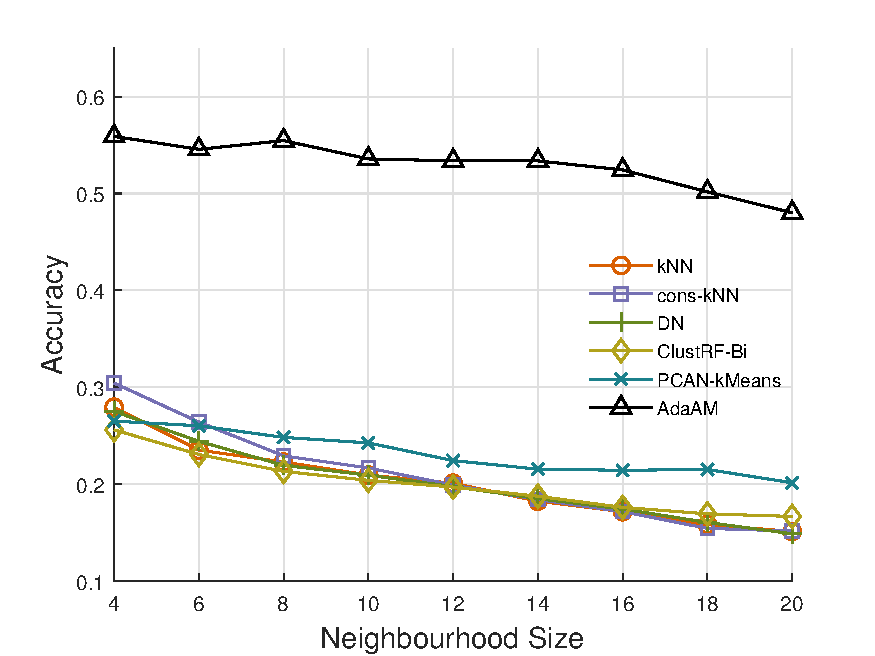
\includegraphics[width=0.9\textwidth]{chap2/sens_ExYaleB1.pdf}}
	\bicaption{在数据集ExYaleB上不同的近邻数量$k$的情况下的算法聚类效果比较}{Clustering results comparison between methods with different neighborhood size $k$ on ExYaleB}
	\label{fig2:Sen3}
\end{figure} 
在聚类效果评估中,我们通过将获得的聚类标签与数据集的真实标注进行比较,使用准确率(accuracy,Acc)来衡量性能。准确率定义如下:
\begin{equation}
	\mathrm{Acc} = \frac{1}{n}\sum^{n}_{i=1}\delta(p_i, map(q_i))
\end{equation}
其中$n$为数据实例数量,$p_i$是数据$x_i$的预测标签,$q_i$为真实标签。当$x=y$时$\delta(x, y) = 1$,否则$\delta(x,y) = 0$。$map(q_i)$表示最佳匹配函数,该函数通过在预测出的类之间交换类标签实现,预测标签与真实标签的最佳匹配。

全部实验都通过MATLAB R2014a实现,并运行在具有Quad Core 3.00 GHz CPU和16 GB内存的Linux系统计算机上。

\subsection{性能评估与比较}
\begin{figure}[t]
	\centering
	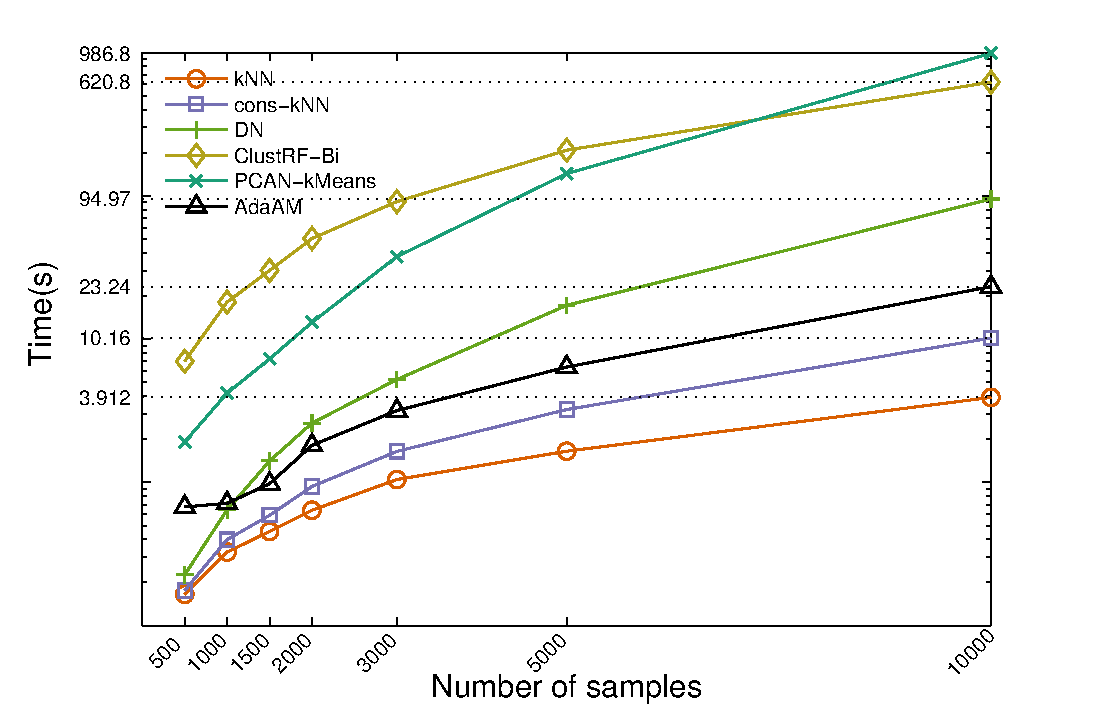
\includegraphics[width=0.9\columnwidth]{chap2/time.pdf}
	\bicaption{不同数据实例数量的情况下六个算法的时间使用比较}{Time consumption of six approaches with different number of data instances}
	\label{fig2:Time}
\end{figure}

在聚类准确率评估的实验中,我们在上述五个基准数据集上对提出的AdaAM方法及其他五种算法进行了数据投影效果的评估。表\ref{tab2:Acc}给出每个模型在100轮$k$-means聚类中聚类预测准确率的平均值和最大值。由于PCAN算法不通过$k$-means聚类而直接产生聚类结果,所有PCAN性能评估结果仅有唯一结果,不存在平均值与最大值。从表\ref{tab2:Acc}中我们可以观察到AdaAM算法在无监督度量学习任务上的优越性。在绝大多数情况下,AdaAM算法的性能明显优于其他方法。我们的方法在五个数据集的平均准确率指标上获得了四个最优,在最大准确率指标上五个全部最优。我们还可以观察到,所提出的AdaAM在ExYaleB数据集上相对其他五种方法具有绝对性优势。与其他数据集不同,ExYaleB中的图像数据已针对人脸进行了较好的对齐,并图片拍摄场景处于不同的光照环境下。这种差异使得相同光照下的图片即使属于不同类别的图像依然具有较大的相似度,从而使数据图上类间连接增多,导致了高秩的相似性矩阵。我们的方法基于最优相似性矩阵的低秩近似,能够有效处理相似性矩阵中的此类噪声。

由于在准确率评估实验中近邻数量$k$选择标准是固定的,这可能会导致算法无法在实验中获得最优性能。因此我们在图\ref{fig2:Sen}、图\ref{fig2:Sen2}及图\ref{fig2:Sen3}中展示了AdaAM与对照算法在五个图像数据上的聚类准确率随近邻数量大小变化的趋势。我们在每个数据集上分别设计了近邻数量从$k=4$到$k=20$、间隔为2的9组实验,以评估不同算法的聚类效果是否会随近邻数量不同,即相似性矩阵的稀疏程度,而产生显著的波动。从图中可以看出,在大多数情况下,AdaAM可取得最佳性能,并且对近邻数量的敏感性与其他模型相当或更低。由于我们的方法基于最佳相似性矩阵的低秩近似,需要更多的成对相似度的信息。因此,对于极小的近邻数量$k$,部分基线方法有时比我们的方法效果更好,这一点可以从图\ref{fig2:Sen2}可以看出。

在图\ref{fig2:Time}中,我们通过半对数图描绘了六种算法在不同数据量的MNIST子集上的运行时间,以此说明AdaAM方法的高效性。 从图中可以看出,我们的方法在实际使用中是一种时间代价较低的算法。相比于PCAN-$k$Means,ClustRF-Bi和DN方法,AdaAM算法的时间消耗要低得多。需要注意的是,$k$-NN作为一个基线算法,本身并不需要进行相似性矩阵学习,因此其所需的运行时间仅包括$k$-NN热力核相似性矩阵构建、LPP线性投影矩阵计算及$k$-means聚类这三种所有对照算法共享的基本操作,所以其计算效率必然最高。我们同时还展示了AdaAM的运行时间大约为Cons-$k$NN的两倍,但在整体性能方面AdaAM相比于其他算法依然具有明显的优势。

\section{本章小结}
在本章中,我们提出了一种用于无监督度量学习的具有创新性的相似性学习方法,称为自适应相似性矩阵(Adaptive Affinity Matrix,AdaAM)。在我们所提出的新的相似性学习模型中,相似性矩阵从与谱聚类相同的计算框架中学习获得的。 更具体地说,我们表明相似性学习可以简化为奇异值分解问题。获得学习到的相似性矩阵后,可以借助于类似LPP这样基于相似性图的现成的算法来学习距离度量。我们所采用的低秩近似的优化方法可以在相似性矩阵学习的过程中进一步提高学习效率。
我们在UMIST、COIL20、USPS、MNIST及ExYaleB五个被广泛使用的图像数据集上对AdaAM及其他对照算法的进行了大量聚类实验。
实验结果证明了所提出的方法AdaAM的性能优越性、稳定性与高效性。